%---------------------------------------------------------------
%---------------------------------------------------------------
\chapter{Generierung von Skeletten}
\label{chapter:skeleton_generation}

\todo{Einleitung}


%------------------------------------
\section{Bestandteile eines Skeletts}

Ein Skelett besteht aus Knochen und Gelenken. Zwei Knochen sind jeweils durch ein Gelenk miteinander verbunden. Im Folgenden werden sowohl Knochen als auch Gelenke genauer beschrieben.

% Knochen
Jeder \emph{Knochen} hat sein eigenes lokales Koordinatensystem und wird zunächst als Quader dargestellt. Der Ursprung des Koordinatensystems befindet sich in einer Ecke des Quaders.
Informationen, die für die Darstellung eines Knochens erforderlich sind, sind also
seine Ausdehnung in alle drei Raumrichtungen (die Kantenlängen des Quaders) und die Position und Orientierung des Ursprungs im globalen Koordinatensystem.

% Hierarchie
Die Knochen sollten eine Hierarchie (einen Baum) bilden, da das von Algorithmen für Animationen so erwartet wird. \todo{Verweis auf previous work, wenn ausgearbeitet} Da der Wirbeltierbauplan aus Abbildung \ref{bauplan_skelett} verwendet wird, ist das auch möglich. Im Allgemeinen ist ein Skelett aber weder zusammenhängend noch ohne Kreise.

% Wurzel
Für eine Hierarchie ist ein erstes Element nötig, die Wurzel des Baums.
Dafür bietet sich ein Knochen in der Nähe des Schwerpunkts an. Oft wird hierfür die Hüfte verwendet. \todo{Beispiel/Quelle}
Da aber nicht jedes Wirbeltier eine Hüfte besitzt und es die Generierung vereinfacht, wird als Wurzelknochen ein Knochen ohne Ausdehnung in der Mitte der Rückenwirbelsäule verwendet. Dieser Knochen wird im Folgenden als \emph{Wurzelknochen} bezeichnet. Liegt Knochen $B$ in der Hierarchie direkt unter Knochen $A$, so ist $A$ der \emph{Elternknochen} von $B$ und $B$ ein \emph{Kindknochen} von $A$.

% Transformationsmatrizen
Es ist sinnvoll für jeden Knochen nicht die Position im globalen Koordinatensystem anzugeben, sondern seine Position im Koordinatensystem des Elternknochens. Verfolgt man den Pfad von einem Knochen zurück zum Wurzelknochen, so kann die Position im globalen Koordinatensystem trotzdem ausgerechnet werden. \todo{Verweis auf IK} \\
Für die Darstellung werden Transformationsmatrizen mit homogenen Koordinaten verwendet. Genauere Informationen zu diesen Transformationsmatrizen und wie sie in verschiedenen Situationen berechnet werden können sind in Absatz \ref{implementation_detail_matrices} zu finden.

% Gelenke
Ein \emph{Gelenk} ist, wie auch in der Natur, ein Verbindungsstück zwischen zwei Knochen. Es legt fest wie die beiden Knochen sich relativ zueinander bewegen können. Im Gegensatz zu echten Gelenken haben Gelenke hier aber keine Ausdehnung. Sie werden am Ende im 3D-Modell nicht dargestellt.\\
Ein Gelenk wird im Koordinatensystem des Elternknochens dargestellt. Es wird beschrieben durch seinen Abstand zum Ursprung des Elternkoordinatensystems und Bewegungseinschränkungen für den Kindknochen. Ein Gelenk kann null bis zwei Freiheitsgrade haben. Bei einem Winkel von $0^\circ$ hat das Kindelement die gleiche Ausrichtung wie das Elternelement. In Abbildung \ref{joints} sind alle Gelenke mit mindestens einem Freiheitsgrad, die im Algorithmus verwendet werden, dargestellt.

% Berechnung Transformationsmatrix des Kindelements
Ist ein Elternknochen mit einem Gelenk in einer bestimmten Ausrichtung gegeben, so lässt sich daraus die Transformationsmatrix des Kindelements berechnen.


%-----------------------------
\section{Aufbau als Grammatik}
\label{section:grammar}



\begin{itemize}
  \item verwende kontextfreie Grammatik, kein L-System (aber Baumstruktur)
  
  \item Aufbau der (Nicht)terminale als Baum
  \item nur Terminale (mit Gelenk) können Kinder haben
  \item Reihenfolge der Anwendung der Regeln sollte beliebig sein
  
  \item Wachstum unter Berücksichtigung verschiedener Randbedingungen wie Bodenposition, Anzahl Extremitäten etc.\
  \item Bounding Box für Nichtterminale ist nicht nötig.
  
  \item Symmetrie der Skelette (spiegle Elemente zum Schluss)
  \item Skelett zusammenhängend und ohne Kreise (Brustbein)
  
  \item am Ende aber für jedes Nichtterminal genau eine Regel
  \item Arme und Beine ähnlich, könnten evtl gleiche Regel benutzen
 \end{itemize}
 
 \begin{sidewaysfigure}
  \centering
  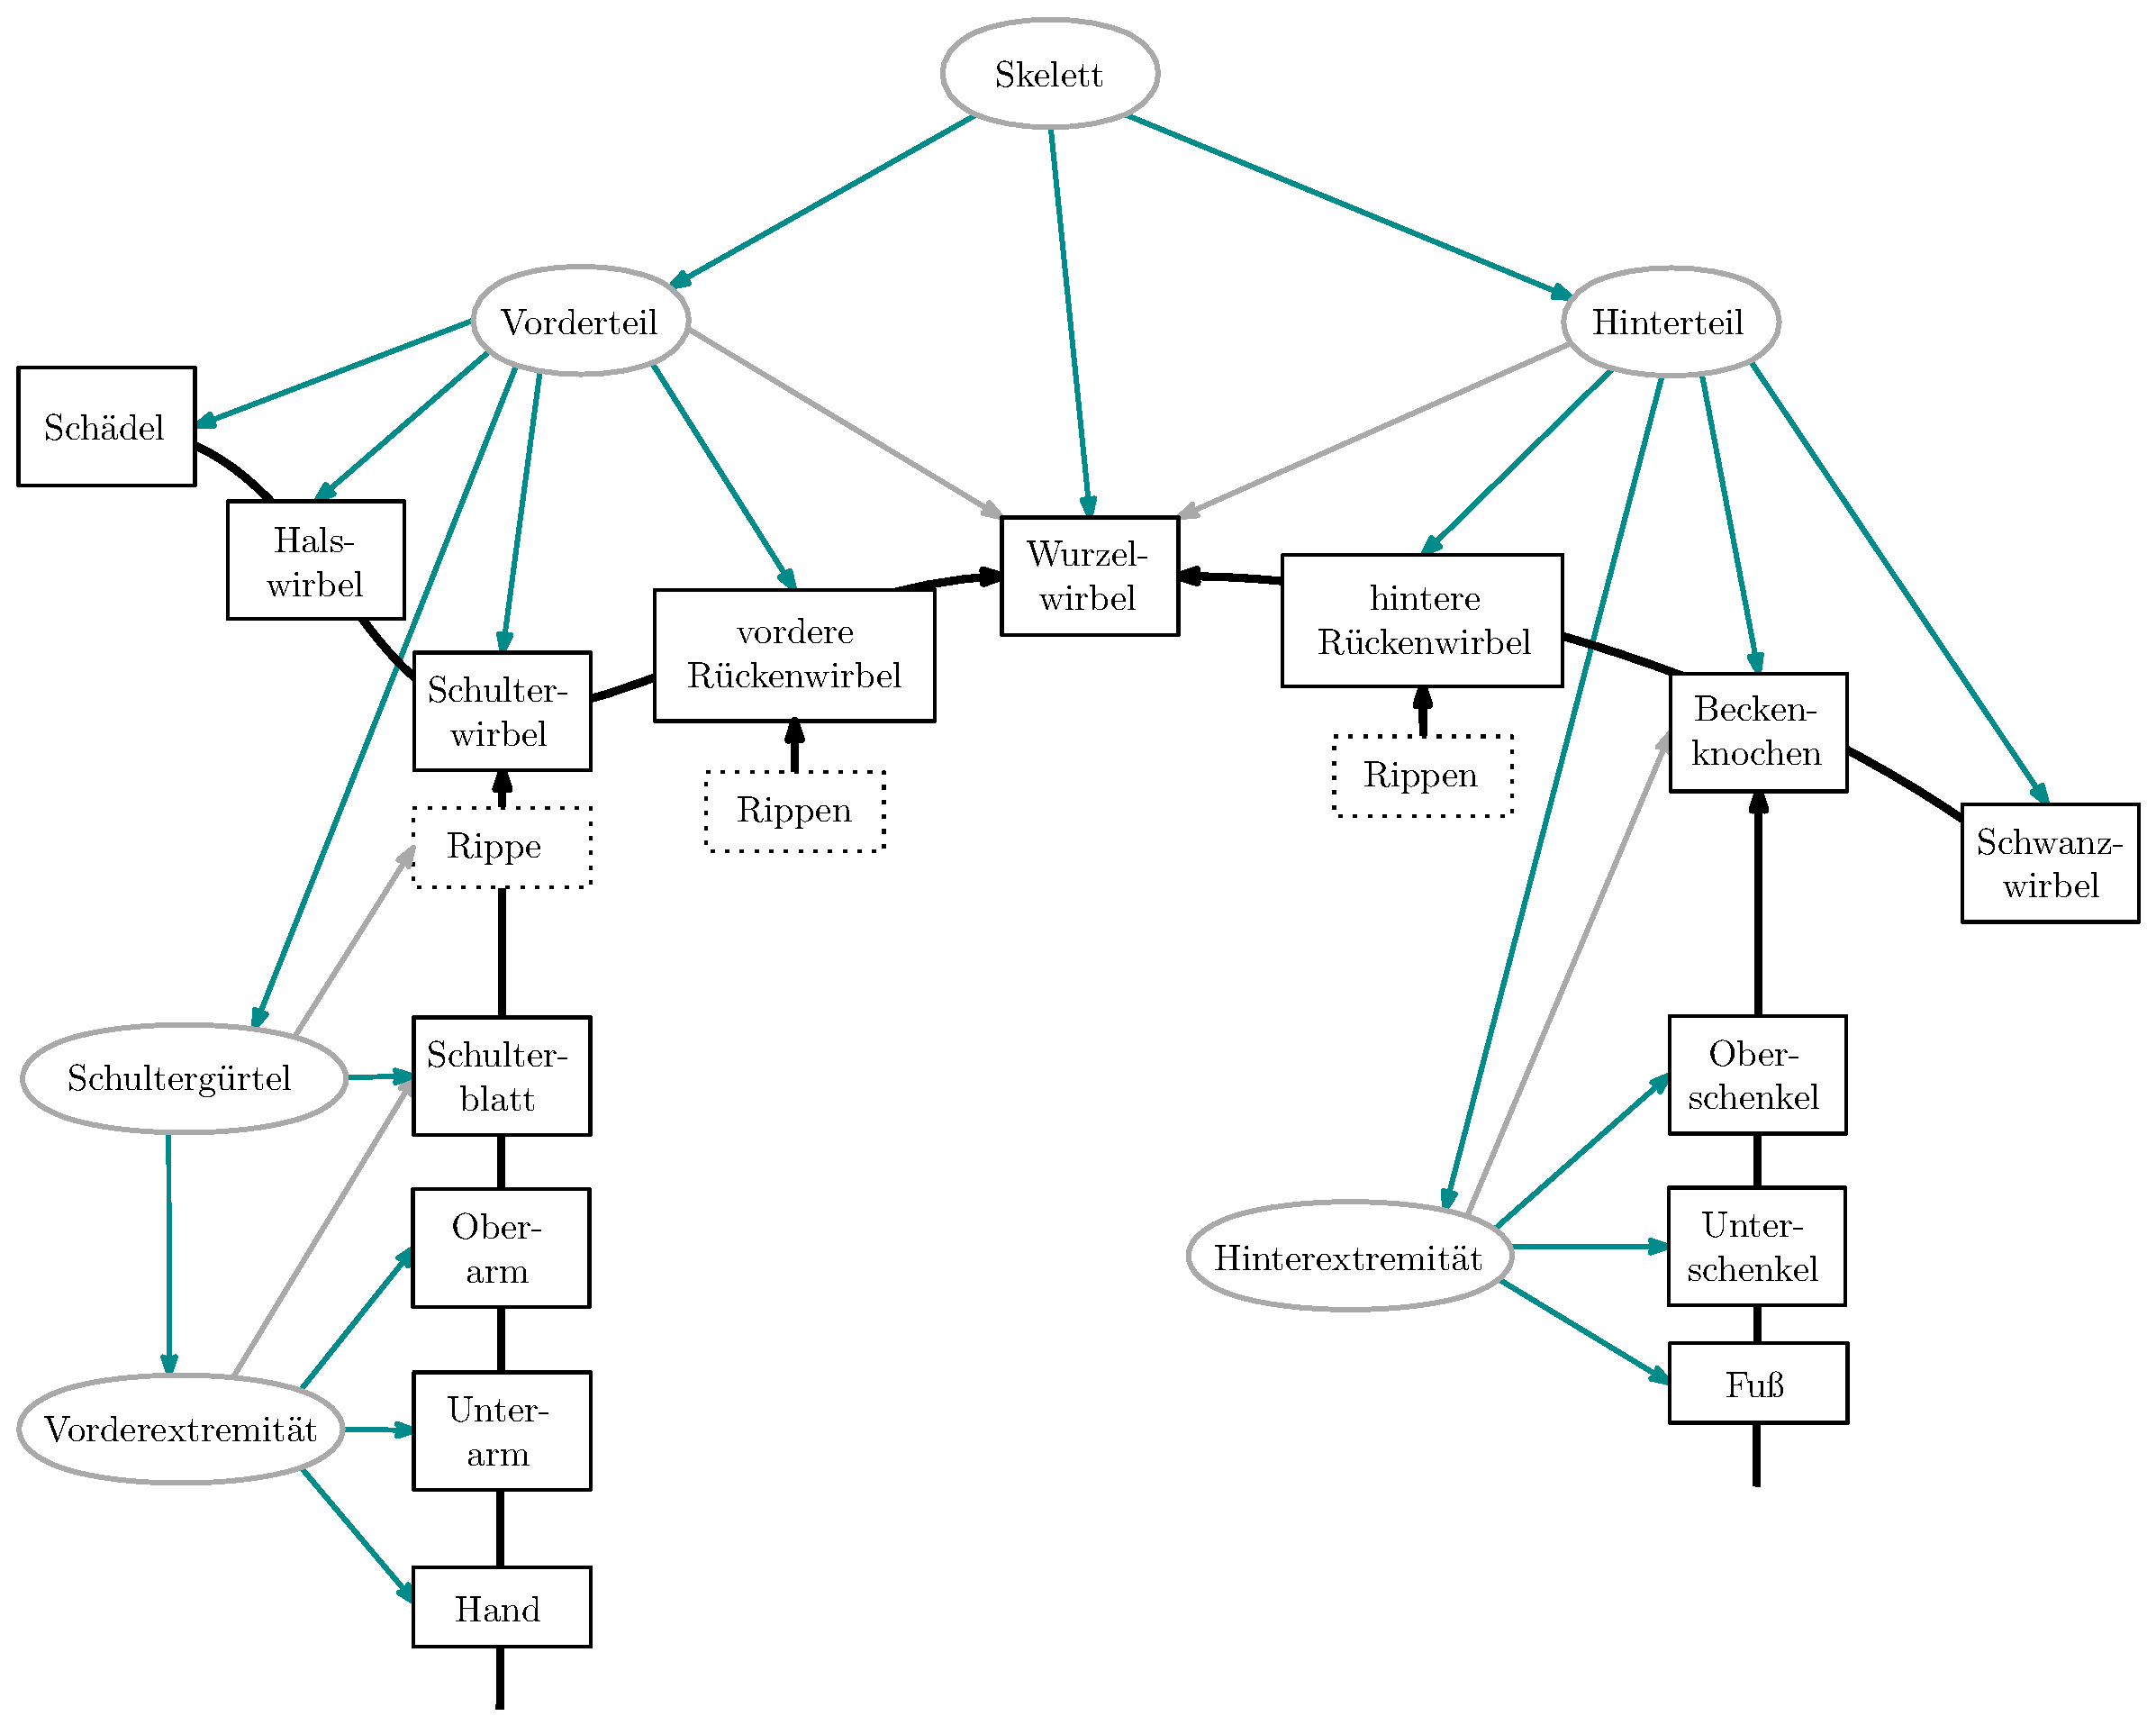
\includegraphics[height=14cm]{graphics/grammarGraph}
  \caption{Aufbau der Grammatik}
  \label{grammar_graph}
 \end{sidewaysfigure}




%--------------------------------------------------
\section{Überblick über den Ablauf der Generierung}

\todo{Koordinatensystem beschreiben, Achsen etc auch für später (zB Beinalgo) festlegen}\\
\todo{"`Kommunikation"' über SkeletonGenerator}

\fbox{
 \begin{minipage}{\textwidth}
  \centering
  \begin{minipage}{0.9\textwidth}
    
    \vspace{0.5cm}
    {\large Generierung eines Skeletts}

    \begin{enumerate}
      \item \textbf{PCA}: Lese die Beispielskelette ein und berechne den Basiswechsel (siehe \mbox{Kapitel \ref{chapter:pca}}).
 
      \item \textbf{Punkt im PCA Raum}: Bestimme einen (bedingt) zufälligen Punkt im PCA-Raum oder verwende einen vorgegebenen.
 
      \item \textbf{Weitere Merkmale}: Bestimme aus den "`Wahrscheinlichkeiten"' für \emph{Flügel} und \emph{Beine mit Bodenkontakt} Anzahl, Art und Ansatzpunkte der Extremitäten (Abschnitt \ref{section:extremity_generation}) und lege fest an welchen Wirbeln Rippen ansetzen (Abschnitt \ref{section:vertebrae_ribs}).
 
      \item \textbf{Ersetzungsregeln}: Starte mit dem Nichtterminal \emph{Skelett} und wende so lange Ersetzungsregeln an bis nur noch Terminale übrig sind (\mbox{Abschnitt \ref{section:grammar}}).
 
      \item \textbf{Spiegelung}: Spiegle alle Elemente, die nicht auf der Wirbelsäule liegen. Das sind Extremitäten, Rippen und Schulterblatt. (Technische Details zur Spiegelung der Transformationsmatrizen sind in Abschnitt \ref{implementation_detail_matrices} zu finden.)
 
      \item \textbf{3D-Modell}: Generiere aus den Abmessungen der terminalen Elemente 3D-Objekte und füge sie zu einem kompletten 3D-Modelle zusammen. Dafür werden bestehende Modelle von echten Knochen oder einfache Quader eingesetzt (siehe Abschnitt \ref{bone_models}).
 
    \end{enumerate}
    \vspace{0.2cm}
    
  \end{minipage}
 \end{minipage} 
}






\begin{itemize}
 \item Bei echten Wirbeltieren gibt es sehr viele verschiedene Arten von Gelenken \cite[Absatz 21.5.2]{Vergleichende_Anatomie}. Der Einfachheit halber werden hier nur Gelenke betrachtet, deren Winkel schon durch den Grundbauplan festgelegt sind (\zb zwischen Wirbeln), und Gelenke in Extremitätenmit einem Freiheitsgrad (\zb an Ellenbogen oder Knie) (näheres zu Gelenken in Extremitäten weiter unten)

 \item Einheiten der PCA für Koordinaten $[0, 1000]$, deshalb sind die Wirbelsäulen der generierten Skelette auch in diesem Rahmen. Blender interpretiert eine Einheit als $1$m. Deshalb wirken sie sehr groß.
 
 \item Die Abmessungen der Knochen in die verschiedenen Richtungen ist bei den meisten Knochen relativ beliebig gewählt und oft auch immer gleich (außer bei Längen, die von PCA vorgegeben sind). Dafür gibt es keine biologische oder anatomische Grundlage. Man könnte hier sicherlich noch mehr machen (mehr Zufall, mehr anatomisch korrekt etc.)
 \todo{in Implementierungsdetails aufzählen was an Abmessungen alles beliebig (oder auch weniger beliebig) festgelegt wurde.}
\end{itemize}

%-----------------------------------------------
\section{Extremitäten}
\label{section:extremity_generation}

Ein Punkt im PCA-Raum gibt schon viele Eigenschaften des zu generierenden Skeletts vor. Zu den Dingen, die noch festgelegt werden müssen, zählen \zb die Anzahl und Anordnung der Wirbel und Rippen und vor allem die Ausrichtung der Extremitäten. 

% was ist schon vorgegeben
Die Bestandteile einer Extremität sind durch den Grundbauplan (Abbildung \ref{bauplan_skelett}) vorgegeben und die Länge der Bestandteile durch die Entsprechenden Merkmale des PCA-Datenpunkts. Die Schwierigkeit besteht nun darin in den entsprechenden Ersetzungsregeln (siehe Abbildung \ref{grammar_graph}) auch die Positionierung vorzunehmen.

% Allgemeine Schwierigkeit Extremitäten zu positionieren
Das Skelett soll in einer Art Ruheposition dargestellt werden. Im Allgemeinen ist aber nicht klar wie die Ruheposition einer Extremität aussieht. Das ist schon allein daran zu erkennen, dass auf Darstellungen von Wirbeltierskeletten Flügel manchmal ausgestreckt und manchmal eingefaltet sind. Auch Beine sind meist so angeordnet, dass es aussieht als würde das entsprechende Tier gerade laufen. Dies ist auf Abbildung \ref{klippschliefer_farbig} am Beispiel des Klippschliefers sehr gut zu sehen.

Wie in Kapitel \ref{chapter:pca} zur PCA schon erwähnt, ist es deshalb auch schwer möglich die Ausrichtung der Extremitäten \bzw die Winkel an den Gelenken als zusätzliche Dimension in den PCA-Raum mitaufzunehmen.

Die Positionierung der Extremitäten bleibt also ein Problem mit unklaren Anforderungen und vielen Freiheitsgraden.

% Einteilung in Kategorien
Ein erster Schritt an das Problem heranzugehen, ist es in kleinere Unterprobleme zu zerteilen.
Extremitäten können anhand ihrer Funktion in vier Kategorien eingeteilt werden:
Flügel, Flossen, Extremitäten mit Bodenkontakt (im Folgenden als Beine bezeichnet), und Extremitäten ohne Bodenkontakt (im Folgenden als Arme bezeichnet).

Für Flügel, Flossen und Arme gibt es keine besonderen Anforderungen außer, dass sie als solche zu erkennen sein sollten. Deshalb werden sie nach folgenden simplen Anweisungen orientiert:
\todo{Beispielbilder?}
\begin{itemize}
 \item Flossen: Ausrichtung gerade nach hinten (orientiert an Welt-x-Achse)
 \item Arme: Der Oberarm zeigt senkrecht nach unten (orientiert an Welt-y-Achse), im Ellenbogengelenk ist ein $90^{\circ}$ Winkel und die Hand verlängert Unterarm nach vorne.
 \item Flügel: Jedes beteiligte Gelenk hat ein Intervall mit festen Grenzen speziell für Flügel, aus dem zufällig ein Winkel gewählt wird.
\end{itemize}

Nun bleibt nur doch die Ausrichtung der Beine, für die die zusätzliche Anforderung gilt, dass sie den Boden berühren sollen.


%- - - - - - - - - - - - - - - - - - 
\subsection{Berechnung der Bodenhöhe}
\label{floor_height}

% Warum nicht Höhe 0?
Zunächst könnte man davon ausgehen, dass der Boden einfach auf Höhe null sein sollte. Das Problem hierbei ist aber, dass die von der PCA berechneten Längen für die Extremitäten meist so kurz sind, dass die Beine dann den Boden nicht mehr erreichen würden. Das liegt daran, dass auf den Bildern, die als Eingabebeispiele für die PCA verwendet wurden, der Boden meistens nicht ganz am unteren Rand ist. Hier würde rigoroses Abschneiden der Bilder auf Fußhöhe wahrscheinlich helfen, es würde in vielen Fällen aber auch ein Großteil der Füße verloren gehen.

% Berechnung
Die Höhe des Bodens wird also anhand der von der PCA generierten Längen der Extremitäten festgelegt.
Theoretisch würde es reichen einfach das kürzeste Bein im komplett ausgestreckten Zustand zu betrachten und den Boden auf die Höhe dessen Endpunkts festzulegen.
Das führt aber zu unnatürlich aussehenden Beinen, da das kürzeste Bein dann genau senkrecht nach unten führen muss um den Boden zu erreichen.

Deshalb wird nur ein bestimmter Anteil der Länge der Beine betrachtet. So wird erzwungen, dass die Beine, wenn sie auf dem neu definierten Boden stehen, auch etwas gekrümmt sind. Dieser Anteil ist in der Implementierung mit $0.8$ festgelegt, lässt sich aber natürlich auch variieren.

Wie in Kapitel \ref{chapter:biology} beschreiben gibt es verschiedene Arten von Füßen. Die oben beschriebene Berechnung geht davon aus, dass der Boden mit der Fußspitze berührt wird. Aber natürlich gibt es auch Wirbeltiere, die mit dem flachen Fuß auf der Erde stehen.
Deshalb wird zusätzlich zur Bodenhöhe noch eine Wahrscheinlichkeit berechnet, dass Verse \bzw Handgelenk den Boden berühren.

Wird die Bodenhöhe nach oben verschoben, weil die Beine insgesamt zu kurz sind, ist diese Wahrscheinlichkeit null.
Sind die Beine so lang, dass schon ohne die Bodenhöhe anzupassen die Verse \bzw das Handgelenk auf den Boden reicht, so ist sie eins.
Ansonsten ist die Wahrscheinlichkeit 
\[\frac{\text{Beinlänge} - \text{Höhe des Extremitätengürtels über }0}{\text{Länge des Fußes}}\]
Wenn es Vorder- und Hinterbeine gibt, so wird für beide diese Wahrscheinlichkeit berechnet und dann der Mittelwert genommen. Denn es ist sinnvoll, dass alle Beine den gleichen Punkt auf den Boden bringen.
Deshalb legt auch das erste Bein, das generiert wird, basierend auf der oben berechneten Wahrscheinlichkeit, fest, welcher Punkt gewählt wird.
\todo{Wann wird welcher Fuß verwendet?}


%- - - - - - - - - - - - - - - - - - - - - - - - -
\subsection{Algorithmus zur Ausrichtung der Beine}
\label{leg_algo}

Eine Herangehensweise dieses Problem zu lösen, wäre inverse Kinematik zu verwenden. 
Da das vorliegende Problem aber recht viele Randbedingungen hat, die ausgenutzt werden können, ist es gar nicht unbedingt nötig einen schwergewichtigen Algorithmus zu implementieren, der ein allgemeineres Problem löst.\\
Hier ist \zb in den allermeisten Fällen klar in welche Richtung ein Gelenk gedreht werden muss um den Fuß dem Boden zu nähern oder ihn vom Boden zu entfernen. Außerdem ist gar kein spezieller Punkt auf dem Boden vorgegeben, der erreicht werden soll.

Deshalb wurde hier ein eigener, recht simpler Algorithmus entwickelt, der auf dieses spezielle Problem angepasst ist.

%Gelenke
Die Gelenke in den Extremitäten werden hier so vereinfacht, dass genau einen Freiheitsgrad haben. Eltern- und Kindknochen sind also auf einer gemeinsamen Ebene festgelegt. Die verwendeten Gelenke mit ihren Einschränkungen sind in Abbildung \ref{joints} zu sehen. Der minimale und maximale Winkel für die Gelenke an Schultblatt und Beckenknochen orientieren sich an der Welt-y-Achse, da außerhalb dieses Bereichts keine sinnvollen Ruhepositionen entstehen würden. \\
% Zweiter Freiheitsgrad
Theoretisch haben das Hüft- und das Schultergelenk nicht nur einen, sonder zwei Freiheitsgrade. Der Oberschenkel lässt sich nicht nur nach vorne und hinten bewegen, sondern auch seitlich abspreizen. Das lässt sich auch leicht als zweite Art von Gelenk im Code abbilden. Allerdings liefert der Algorithmus dann oft seltsam anmutende breitbeinige Tiere.
Deshalb wurde der zweite Freiheitsgrad hier außen vor gelassen.
Obwohl es natürlich in der Natur auch viele Tiere mit nach außen gestellten Beinen gibt, wie \zb Echsen.
% + max angewinkelte Pos komisch und Drehrichtung ändert sich je nach anderen Winkel


\begin{figure}
  \subfloat[Vorderextremität]{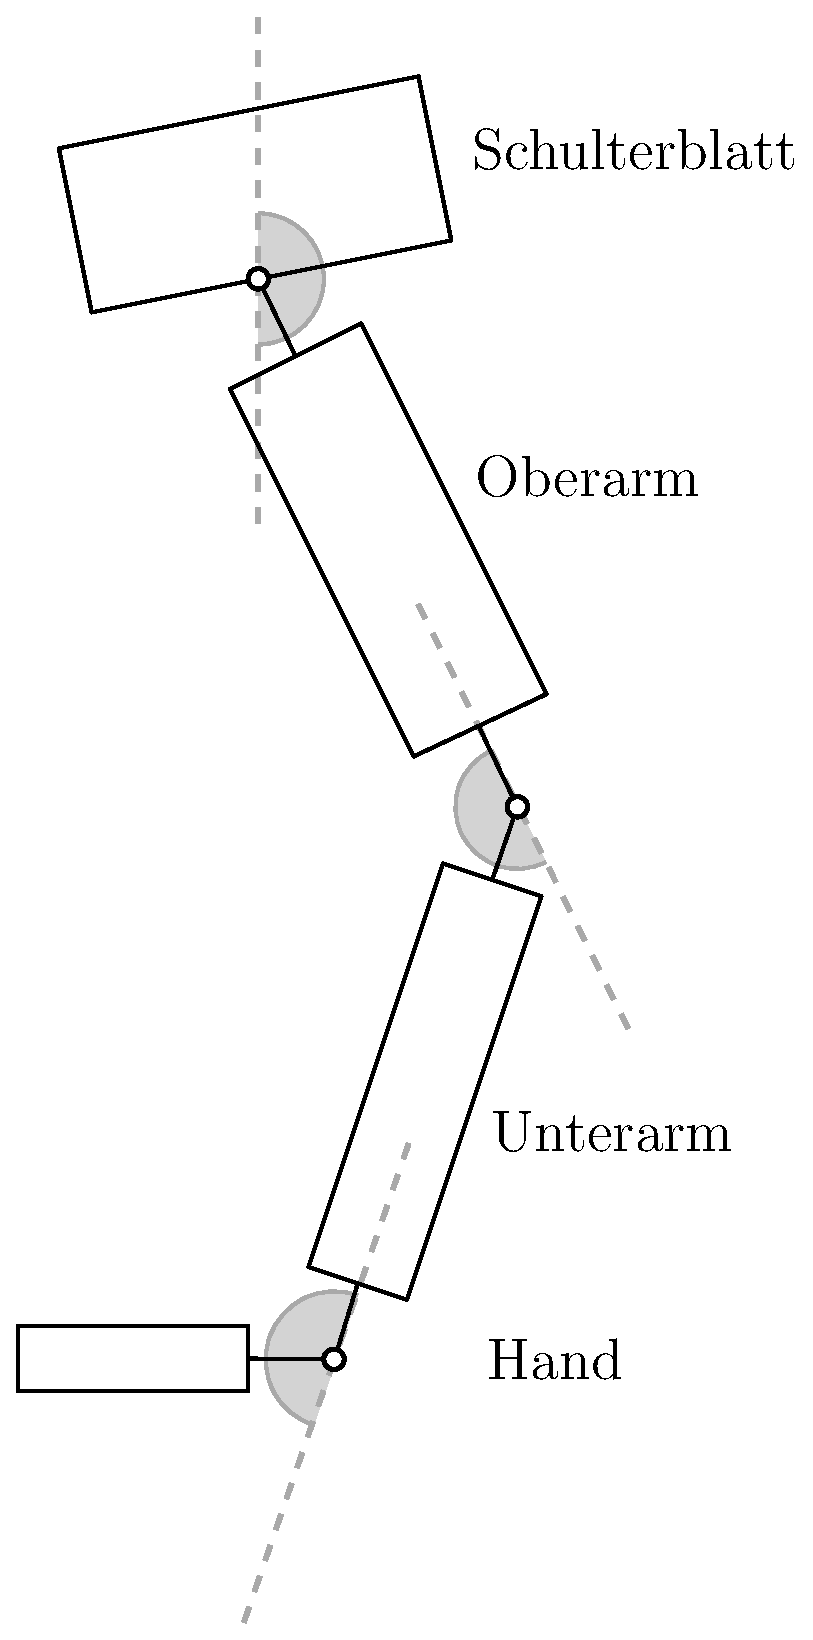
\includegraphics[height=0.4\textheight]{graphics/armJoints}}
  \hfill
  \subfloat[Hinterextremität]{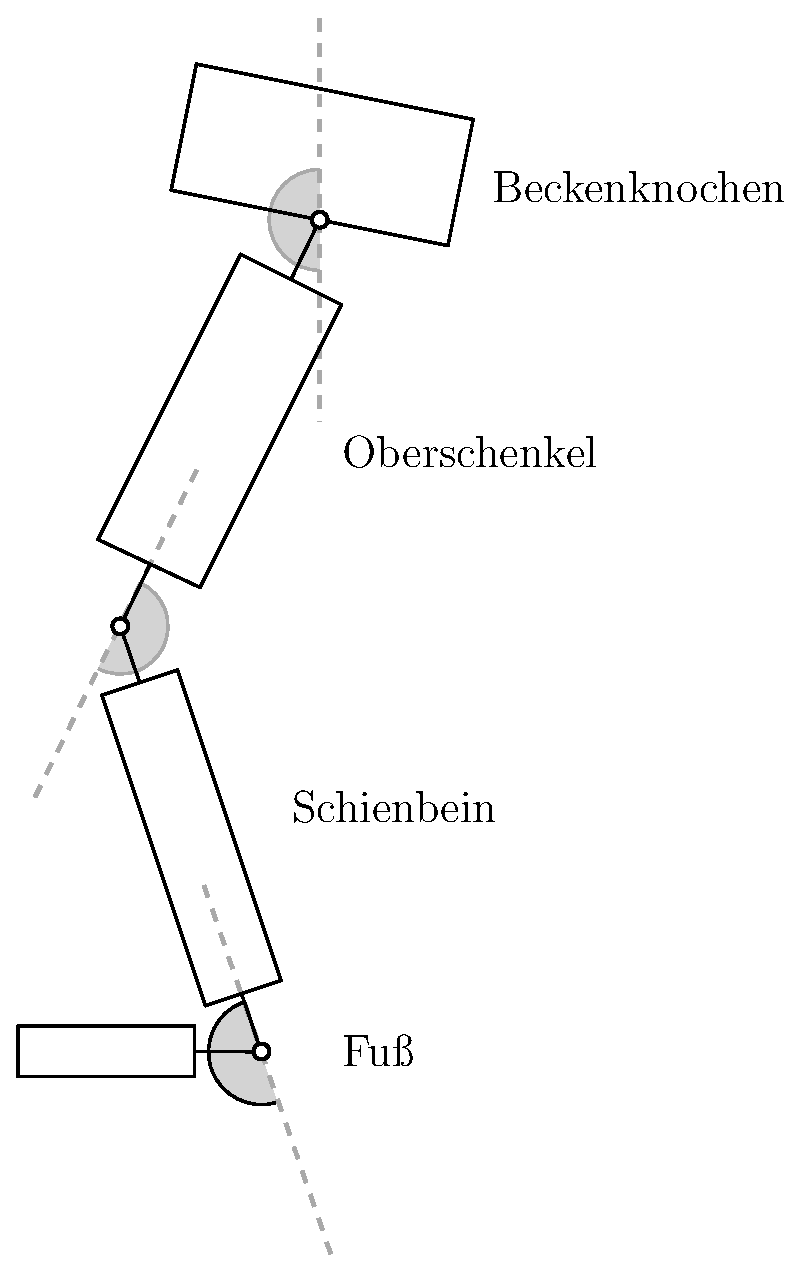
\includegraphics[height=0.4\textheight]{graphics/legJoints}}
  
  \caption{Visualisierung der Bewegungsradien für die Gelenke in Extremitäten mit Bodenkontakt. Darstellung in Seitenansicht (wie in Abbildung \ref{bauplan_skelett}). Die grauen Halbkreise zeigen die möglichen Winkel für eine Ruheposition des Skeletts. Unterarm, Unterschenkel und Fuß können jeweils maximal die Verlängerung des darüberliegenden Knochens bilden und minimal komplett an ihm anliegen. Oberarm und Oberschenkel können nicht über die Senkrechte hinaus gedreht werden.}
  \label{joints}
 \end{figure}


% \begin{algorithm}
%  \caption{Beinalgorithmus}
%  \label{beinalgo}
%  
%  \begin{algorithmic}
%     \STATE{step = 0\\
%     maxSteps = 50\\
%     angleStepSize = $40^\circ$}
% 
%     \WHILE{floor not reached and step < maxSteps}
%         \FORALL{joints}
%             \IF{child bone of joint has not reached floor and movement nearer to floor possible}
%                 \STATE try change joint angle
%             \ENDIF
%         \ENDFOR
%         \IF{angleStepSize > eps}
%             \STATE reduce angleStepSize
%         \ENDIF
%     \ENDWHILE
%  \end{algorithmic}
% \end{algorithm}
\todo{Pseudocode?}

% iterativ, Drehrichtung
Der Algorithmus geht iterativ vor.
In jedem Schritt wird für jedes Gelenk berechnet ob sein Winkel vergrößert oder verkleinert werden muss um den dazugehörigen Knochen näher zum Boden zu bewegen.
Mit dem "`dazugehörigen"' Knochen ist hier derjenige der beiden an das Gelenk anschließenden Knochen gemeint, der das Kindelement des anderen ist.
Die Drehrichtung lässt sich relativ leicht herausfinden indem die Ausrichtung des Knochens mit der Welt-y-Achse verglichen wird. Je senkrechter der Knochen ausgerichtet ist, desto ausgestreckter ist das Bein.
Es gibt also globale Randbedingungen und lokale Einschränkungen je nach Gelenk. % Problematik mit lokalen Winkelkonstraints vs. globalen Berechnungen für Abstand zum Boden?

% Startposition, Bewegungseinschränkungen
Die Startposition der Extremität ist maximal angewinkelt. Die Gelenke beginnen also mit ihren kleinst- \bzw größtmöglichen Winkeln. In den folgenden Iterationen wird dann derjenige Endpunkt der Extremität dem Boden genähert, der zum Schluss Bodenkontakt haben soll. \todo{würde wahrscheinlich auch mit ausgestrecktem Bein als Startpos gehen; was wäre dabei zu beachten}
Ohne weitere Einschränkungen kann es nun passieren, dass unnatürliche Positionen auftreten, in denen \zb der Fußspann näher am Boden ist als die Fußsohle.
Oder es kann passieren, dass ein Knochen über die positive Welt-y-Achse hinaus gedreht wird. Das Problem dabei ist, dass die Einschränkungen an den Gelenken nicht zulassen, dass der Knochen sich unbegrenzt in diese Richtung weiterdreht und der Knochen dann "`feststeckt"'. Deshalb wird nach jeder Drehung festgestellt ob so eine Situation eingetreten ist und wenn ja, wird die Drehung rückgängig gemacht.
Die Drehung wird ebenfalls rückgängig gemacht, falls sie bewirkt, dass die Knochen unterhalb der Bodenhöhe landen.
\todo{Beispielbilder}
So ist zu jeder Zeit garantiert, dass die Knochen auf der "`richtigen"' Seite der y-Achse liegen und nicht unterhalb der Bodenhöhe sind. % Invarianten

% Verkleinerung der Größe der Drehwinkel
In jeder Iteration werden die Winkel, um den die Gelenke gedreht werden, um einen bestimmten Anteil verkleinert. Zu Beginn soll, mit großen Veränderungen, eine grobe Ausrichtung der Gelenke vorgenommen werden, die dann immer weiter verfeinert wird.
Der Startwinkel darf nicht zu klein sein, weil die Gelenke sonst ihre Zielpositionen nicht erreichen können. Ist der Startwinkel allerdings zu groß, bewirkt es in vielen Fällen nur, dass die Drehung nicht durchgeführt werden kann, weil die oben genannten Randbedingungen verletzt werden.\\
Die Verkleinerung des Winkels darf nicht zu schnell geschehen, weil dann wiederum die Endposition nicht erreicht werden kann. Wenn sie aber zu langsam geschieht passiert in vielen Schritten wiederum nichts wegen verletzter Randbedingungen.\\
Durch Ausprobieren wurden folgende Zahlen als sinnvoll erachtet: Startwinkel $40^{\circ}$, später dann jeweils $\frac{6}{7}$ davon.

Falls sich der Abstand zum Boden kaum verändert, liegt also die Vermutung nahe, dass die Gradzahl zu groß ist und deshalb alle möglichen Winkeländerungen invalide sind. Deshalb wird in diesem Fall die Gradzahl für die nächste Iteration stärker verkleinert (halbiert).

\todo{Wkten für Gelenke, Vorteil?}

% Probleme bei sehr kurzen Beinen
Treten sehr kurzen Beinen auf, hat der Algorithmus außerdem einige kleine Probleme. Diese werden genauer in Abschnitt \ref{leg_positioning_short_legs} beschrieben. Da die Beine aber in diesen Fällen, wie gesagt, sehr kurz sind, ist es für den Gesamteindruck gar nicht besonders wichtig wie genau sie angeordnet sind.

% Vergleich echter und generierter Beinstellungen
Wie in Kapitel \ref{chapter:additional_features} beschrieben, lassen sich auch die Eingabebeispiele der PCA laden. Bei ihnen sind dann alle Attribute, die die PCA liefert, schon festgelegt. Alle anderen müssen jedoch noch generiert werden.
Dazu gehören auch die Beine.
Vergleicht man nun die Beinstellung, die der oben beschriebene Algorithmus generiert, mit der Beinstellung auf dem Eingabebild, lassen sich teilweise sehr große Unterschiede feststellen. \todo{gutes und schlechtes Beispiel (schlecht: Brachiosaurus, Elefant)}

% Mehr Infos nötig für Verbesserungen
Um in allen Fällen eine realistisch wirkende Positionierung der Beine zu bekommen, müsste noch sehr viel mehr Arbeit in den Algorithmus gesteckt werden. Außerdem bräuchte der Algorithmus mehr Informationen zum Tier. Solche Zusatzinformationen könnten beispielsweise die Art des Fußes oder die Fortbewegungsart sein. Auch könnte es helfen, wenn es eine sinnvolle Möglichkeit gäbe die Winkel an den Gelenken als Dimension für die PCA mitaufzunehmen. Dafür müsste man sich aber, wie zu Beginn des Kapitels schon erwähnt, auf eine kanonische Ruheposition einigen und dann auch noch Beispiele in genau dieser Position finden.

% für Weiterverwendung werden Beine sowieso angepasst
Ein fertig generiertes Skelett wird höchstwahrscheinlich auch noch "`weiterverarbeitet"'. Soll \zb ein animiertes Tier daraus werden, so müssen Bewegungszyklen geschaffen werden. Dafür muss jedes Gelenk vielfach bewegt werden. Soll ein Tier mit Haut und Muskeln daraus werden, so müssen Muskeln an den Knochen ansetzen, die dann einen nicht unerheblichen Anteil an der Positionierung der Beine haben.

% Beinalgo nicht weiter anpassen
Die von dem hier beschriebenen Algorithmus generierte Position kann also gut als erster Eindruck dienen muss aber in den meisten Fällen noch angepasst werden. Ausgehend von der gegebenen Datenlagen und von den zu erwartenden Anwendungen ist es aber nicht sinnvoll den Algorithmus weiter zu verfeinern.

%--------------------------------------
\subsection{Zusätzliche Ansatzpunkte für Extremitäten}

Ansatzpunkte für Extremitäten sind natürlich zunächst der Hüftgürtel und der Schultergürtel. Um auch die Generierung fantastischer Tiere (siehe Abschnitt \ref{biology_mythology}) zu ermöglichen, ist es aber möglich dies zu erweitern.

% 2 Extremitäten an einem Gürtel
Eine einfache Möglichkeit ist hier zunächst die Anzahl der möglichen Extremitätenpaare von zwei auf vier zu erhöhen, indem einfach an der Hüfte und der Schulter jeweils zwei Paare ansetzen dürfen. Dafür wurden an der Hüfte \bzw der Schulter mehrere Gelenke direkt hintereinander angelegt, an denen Extremitäten ansetzen können. Das ermöglicht beispielsweise Tiere wie den Pegasus.\\
% Keine Flügel und Arme an der Hüfte
Flügel und Arme dürfen hierbei weiterhin nur an der Schulter ansetzen, Beine und Flossen an beiden Stellen. Der Grund dafür ist, dass die meisten generierten Skelette seltsam wirken, wenn an der Hüfte Flügel oder Arme ansetzen und dafür an der Schulter Beine beginnen. Das liegt daran, dass existierende Tiere mit Flügeln oder Armen ihren Schwerpunkt im hinteren Bereich haben und sie auf den Hinterbeinen stehen. Deshalb wird die Wirbelsäule durch die PCA auch dementsprechend angelegt.

% mehr Extremitätengürtel auf dem Rücken
Eine Überlegung war auch zwischen Schulter und Hüfte weitere Extremitätengürtel anzubringen, um \zb Tiere wie asiatische Drachen erzeugen zu können. Das stellt sich aber als schwierig heraus. Die Wirbelsäule ist zwischen Hüfte und Schulter meist nach oben geschwungen und im Bauchraum befinden sich die meisten Organe des Tieres. Ein zusätzlicher Extremitätengürtel würde den Bauchraum einschränken. Außerdem wirkt dann auch die nach oben geschwungene Wirbelsäule anatomisch seltsam.
"`Verdoppelt"' man die Schwingung der Wirbelsäule und hängt einfach einen weiteren Rücken hinten oder vorne an, so wirkt es ebenso seltsam, da dann die "`Höcker"' der Wirbelsäule für das Tier wahrscheinlich nicht wirklich ein Vorteil sind und nur die Fortbewegung erschweren.
Asiatische Drachen sind ein "`Spezialfall"'. Sie besitzen langen, schlangenartigen Körper, bei dem die Wirbelsäule gerade verläuft. Deshalb treten die oben genannten Probleme bei ihnen nicht auf.

% zweiter Schultergürtel
Eine weitere Idee, die auch umgesetzt wurde, ist, eine Art Zentauren zu ermöglichen. Hat das Tier einen Hals, der lang genug ist, kann darauf ein weiterer Schultergürtel kurz unterhalb vom Kopf angebracht werden. An diesem Schultergürtel dürfen dann alle Arten von Extremitäten außer Beinen ansetzen. Das wirkt tatsächlich meist auch anatomisch einigermaßen sinnvoll.\\
Ein solcher Schultergürtel wirkt aber nur sinnvoll, wenn auch der Hals lang genug ist. Deshalb wird die Benutzereingabe, die einen zweiten Schultergürtel erzwingt in eine Bedingung für die Halslänge umgewandelt und an die PCA weitergegeben. Gibt es keine Benutzereingabe, so wird ein zweiter Schultergürtel nur generiert, wenn der Hals lang genug ist.

%----------------------------------- 
\subsection{Anordnung und Anzahl der Extremitäten}

Ein PCA-Datenpunkt stellt die Länge der Vorder- und Hinterbeine, die Wahrscheinlichkeit für Flügel und die "`Wahrscheinlichkeit"' für Beine zur Verfügung.
Die genaue Anzahl (auch für fantastische Tiere) und die Anordnung müssen noch festgelegt werden.

Die Position jeder Extremität wird zufällig aus der Menge der möglichen Positionen gewählt. Beine dürfen nicht am zusätzlichen Schultergürtel am Hals generiert werden, Arme und Flügel dürfen nicht an der Hüfte generiert werden und Flossen sind überall erlaubt.\\
Ist für eine Extremität kein Platz mehr, wird zunächst getestet, ob eine der anderen Extremitäten an ihre Position wechseln kann um Platz zu schaffen. Erst wenn das fehlschlägt kann die betreffende Extremität nicht platziert werden.\\
Da die Positionen nicht deterministisch gewählt werden, kommt es bei Tieren mit mehreren möglichen Anordnungen zu unterschiedlichen Ergebnissen bei gleicher Eingabe.

Die Anzahl und Art der Extremitäten orientiert sich zunächst an Benutzereingabe. Gegebenenfalls wurden diese Eingaben auch schon als Bedingungen an die PCA weitergeleitet (siehe Abschnitt \ref{pca_conditions}).

Falls es keine Benutzereingabe für eine Art von Extremitäten gibt, so wird zunächst getestet ob es noch Platz gibt für diese Art. Falls noch Platz vorhanden ist, wird je nach Art unterschiedlich vorgegangen:
Die Anzahl der Beine oder Flügel wird anhand der Wahrscheinlichkeiten des PCA-Datenpunktes generiert, aber maximal ein Paar pro Schulter- und Hüftgürtel. Die "`Wahrscheinlichkeit"' der Beine liegt im Intervall $[0, 2]$. Hier wird, je nach dem ob die "`Wahrscheinlichkeit"' in $[0, 1]$ oder in $[1, 2]$ liegt, ausgelost ob null oder ein \bzw ein oder zwei Beinpaare generiert werden.\\
Für Arme und Flossen gibt es keine Anhaltspunkte durch die PCA. Deshalb wurde einfach festgelegt, dass Arme, wie Flügel, mit der PCA-Flügelwahrscheinlichkeit generiert werden. Beine werden ganz zum Schluss in noch komplett leeren Extremitätengürteln generiert, falls die Länge der dort zu generierenden Extremitäten nicht zu lang ist.

\todo{nachträgliche Umverteilung der Extremitäten sinnvoll? (leere Gürtel auffüllen)}

Dieses Vorgehen führt dazu, dass, wenn ein PCA-Beispiel geladen wird, die Anzahl, Art und Position der Extremitäten nicht unbedingt dem realen Tier entsprechen muss.
Zunächst kann es einen zusätzlichen Schultergürtel geben, falls der Nutzer das erlaubt und der Hals lang genug ist, und es können mehrere Extremitäten pro Extremitätengürtel platziert werden, wenn das erlaubt ist.\\
Die Anzahl der Flügel und Beine wird stimmen, da ihre Wahrscheinlichkeiten ja festgelegt sind, aber ihre Position wird zufällig bestimmt, falls möglich.  Arme und Flossen werden nach den oben genannten Kriterien generiert, falls der Nutzer nichts anderes vorgibt.\\
Wenn ein Tier also möglichst genau reproduziert werden soll, sollte zumindest die Anzahl der Arme und Flossen angegeben werden und ein zweiter Schultergürtel und mehrere Extremitäten pro Gürtel verboten werden.


%---------------------------------------------------
\section{Wirbel und Rippen}
\label{section:vertebrae_ribs}

Weitere Dinge, die festgelegt werden müssen, ist die Anzahl der Wirbel auf den einzelnen Teilen der Wirbelsäule und die Anzahl der Rippen.

Die Anzahl der Wirbel orientiert sich an echten Wirbeltierskeletten (siehe Absatz \ref{biology_skeleton}). Auf dem Hals werden $7$ Wirbel generiert, außer das Tier hat Flügel, dann liegt die Anzahl zwischen $10$ und $30$. Auf dem Rücken liegen $25$ Wirbel und auf dem Schwanz $5$ bis $20$.
 Da der "`Wurzelwirbel"' in der Mitte der Rückenwirbelsäule liegt (oder zumindest ungefähr, da Bezierkurve bei $0,5$ ausgewertet bei wird) werden $13$ Wirbel auf der vorderen Hälfte und $12$ hinten generiert.

Eine Bézierkurve ist ein Weg im $\mathbb{R}^2$. Sie ist parametrisiert auf $[0, 1]$ und im Allgemeinen nicht nach Bogenlänge parametrisiert. Das heißt die Geschwindigkeit, mit der die Kurve durchlaufen wird, ist nicht konstant. Wertet man die Kurve also bei $0.5$ aus, wurde nicht notwendigerweise die Hälfte der Strecke zurückgelegt.\\
Für die Generierung von $n$ Wirbeln wurde die Kurve einfach an den Stellen $\frac{i}{n}$ ausgewertet, für $0 \leq i \leq n$. Durch den oben genannten Effekt variiert dann die Länge der Wirbel über den Kurvenverlauf.

Wird die Bézierkurve $B$ nach Bogenlänge umparametrisieren, so erhält man die Kurve $S$ mit:

\[S(t) = \int_0^t \| B'(s) \| ~\mathrm{d}s \]

Das obenstehende Integral ist jedoch schwer zu berechnen, da im Allgemeinen keine Stammfunktion des Integranden zur Verfügung steht. Es gibt jedoch numerische Methoden, mit denen das Problem gelöst werden kann. \cite{ArcLengthParametrization}

Betrachtet man echte Wirbeltiere, so sind keine einfachen Regeln für die Länge ihrer Wirbel ersichtlich. Es gibt beispielsweise eine Studie, die die Beschaffenheit der  Wirbel von Mäusen untersucht \cite{MouseVertebrae}. In dieser Studie auf Abbildung $5$, Seite $19$, ist sehr gut zu sehen, dass die Länge der Wirbel im Verlauf der Wirbelsäule sehr stark schwankt.



Die Anzahl der Rippen und auch die Ausdehnung des Brustkorbs variiert zwischen Wirbeltieren sehr stark. Es gibt Tiere, die an jedem Wirbel der Rückenwirbelsäule Rippen haben und es gibt Tiere die haben nur ein paar wenige auf dem vorderen Teil.
\todo{Beispiele}\\
Deshalb wird ein zufälliges Intervall $[0, x]$ auf der Bézierkurve des Rückens bestimmt. Jeder Wirbel, der in diesem Intervall liegt, bekommt auch eine Rippe.
\todo{Bestimmung der Rippenlänge beschreiben?}


%-----------------------
\section{Knochenmodelle}
\label{bone_models}

Zunächst wird jeder terminale Knochen durch seine Bounding Box dargestellt.
\todo{es sind nicht wirklich Bounding Boxen, eher "`Proxyboxen"'}
Diese Boxen lassen sich aber leicht durch die 3D-Modelle der entsprechenden Knochen ersetzen. Dazu müssen die 3D-Modelle nur im .obj-Format vorliegen und folgenden Bedingungen entsprechen:

Das Modell ist korrekt an den Achsen ausgerichtet und so verzerrt, dass es einen Würfel mit 1(m) Kantenlänge in jeder Richtung möglichst gut ausfüllt.

Lässt man es hierbei bewenden, so ist es relativ schwierig herauszufinden wie man die einzelnen Knochen skalieren muss, dass sie an den Gelenken gut zusammenpassen. Außerdem ist es aufwändig herauszufinden wo die Gelenke an den Knochen ansetzen.

Setzt man sich dagegen etwas über den Gedanken der "`Bounding Box"' hinweg, so kann die Positionierung und Skalierung einfacher werden. Hier wurden, je nach Knochen, einige der folgenden Punkte umgesetzt. \todo{Beispielbilder}
\begin{itemize}
 \item Kleine Fortsätze, die nicht wirklich zur (optischen) Größe des Knochens beitragen, \zb die Fortsätze der Wirbel, ragen aus der Bounding Box heraus.
 
 \item Kantenlängen, die von "`außen"' vorgegeben werden, sind genau auf die Kantenlänge der Box skaliert (also 1). So beispielsweise die x-Länge der Wirbel, die auf der Wirbelsäule genau aneinender stoßen sollen. Dies können aber auch Längen sein, nur einen Teil des Knochens betreffen. Der Beinabstand an der Hüfte ist \zb kleiner als die komplette Breite der Hüfte. Es ist aber einfacher den Beinabstand anzugeben, als die Hüftbreite. Auch die Skalierung der Hüfte in x-Richtung ist zunächst nicht klar, aber wenn die Breite der zugehörigen Wirbel gegeben ist, ist auch klar, wie breit die Hüfte sein soll. Deshalb ist die Hüfte in x-Richtung so skaliert, dass der Teil, an dem der Wirbel ansetzt, schon die komplette Kantenlänge des Würfels ausfüllt. Bei Gelenken, die von der Breite her zusammenpassen sollen, ist dies auch sehr hilfreich. Aber das führt natürlich auch dazu, dass die "`Bounding Box"' nicht mehr viel mit der resultierenden Größe des Knochens zu tun haben muss.
 
 \item Kantenlängen, die nicht vorgegeben werden, sind einfacher passend zu bestimmen, wenn sie nicht komplett unabhängig von den anderen Raumrichtungen sind. Ist \zb die x- und y-Skalierung eines Knochens vorgegeben, und die Skalierung in z-Richtung soll nur möglichst gut dazu passen, so ist es sinnvoll, das 3D-Modell schon so zu speichern, dass die z-Richtung von einer der anderen Richtungen abhängt. Tut man dies nicht, so führt das relativ leicht dazu, dass die Knochen grundlos verzerrt werden.
 
 \item Längen die variiert werden können sollen \zb die Länge der Wirbel oder der Beinabstand der Hüfte sollten genau eine Kantenlänge der 1x1 Box einnehmen.
\end{itemize}
\todo{Schwierigkeit bei stark gebogenen Knochen}

Liegen die Modelle in diesem Format vor, können sie einfach eingelesen werden und anhand der Skalierung der Bounding Box skaliert werden.
Hier wurden vor allem Modelle von menschlichen Knochen verwendet, da sie leichter verfügbar sind. Manche Knochen sind jedoch auch von anderen Tieren. Das führt \zb bei dem verwendeten Unterarmknochen des Pferdes dazu, dass er etwas überdimensionierte Fortsätze am Ellenbogen bekommen, wenn man ihn großskaliert. Das liegt daran, dass dieser Knochen beim Pferd eigentlich relativ kurz ist.

% Ausrichtung der Knochen
Eine Schwierigkeit daran Modelle in der oben genannten Form herzustellen ist, dass nicht unbedingt sofort klar ist, wie die Knochen ausgerichtet werden müssen. Die Hüfte muss \zb so ausgerichtet werden, dass der Anfangs- und Endpunkt der durchgehenden Wirbelsäule auf gleicher Höhe liegen, damit nachfolgende Wirbel auch richtig anschließen. (Das funktioniert natürlich nur, weil die Wirbelsäule an der Stelle der Hüfte quasi gerade ist.) \todo{wg Lizenz Pferdehüfte verwendet, die nicht mit Wirbelsäule verwachsen ist}
Auch die Positionierung der Rippen und des Oberarms in Kombination mit dem Unterarm ist anspruchsvoll. Dabei hilft es 3D-Modelle zu haben, in denen die anderen Knochen auch schon vorhanden sind, um sich die Ausrichtung abzuschauen. Außerdem können Bilder von Skeletten zu Rate gezogen werden. Und zuletzt muss man die genaue Positionierung einfach testen.

% Gelenke korrekt ausrichten
Zusätzlich muss beachtet werden wie die Knochen aneinander anschließen \bzw wie sie für die entsprechenden Gelenke korrekt positioniert sind. Das erfordert etwas "`finetuning"'. Für jeden Knochen sind dafür in Abhängigkeit zur Bounding Box zwei Offsets gespeichert: das Offset zu dem Gelenk, das ihn mit seinem Elternknochen verbindet und das Offset zu dem Gelenk, das ihn mit seinem Kindknochen verbindet (oder mehrere, falls vorhanden). Dies sorgt dafür, dass die Positionierung der Knochen stimmt, egal wie groß sie sind. Ist ein Knochen sehr groß und ein anschließender sehr klein (oder anders herum), so kommt es natürlich trotzdem vor, dass die Gelenke nicht wirklich ineinander passen. Für solche Situationen bräuchte man verschiedene 3D-Modelle, die je nach Gegebenheit eingesetzt werden.

% Köpfe
% Köpfe sind kompliziert $\rightarrow$ Auswahl an Köpfen bereitstellen (evtl. leicht skalier-/verformbar oder ineinander überführbar)
Da der Kopf \bzw der Schädelknochen im Gegensatz zu anderen Knochen bei Wirbeltieren sehr stark variiert, ist es sinnvoll mehrere Schädelknochen zur Auswahl zu haben. Geht die Menge an verfügbaren Schädelknochen über "`Tier mit Flügeln"' und "`Tier ohne Flügel"' hinaus, so ist es außerdem sinnvoll die Auswahl des passenden Schädelknochens dem Nutzer zu überlassen.



% Hände und Füße
Bei Händen und Füßen ist das Problem ebenso, dass es sehr viele verschiedene Ausprägungen davon gibt. Hier lassen sie sich jedoch grob nach Extremitätentyp unterscheiden. Diese Unterscheidung kann aber beliebig fein sein. Hier wurde nur nach Flügel, Flosse \todo{?} und Extremität mit Bodenkontakt unterschieden. Und bei Extremitäten mit Bodenkontakt wurde nochmals danach unterschieden wie flach der Fuß oder die Hand auf dem Boden aufkommt (bei weniger als $45^\circ$ ist es eine menschliche Hand, sonst ein Huf). \todo{ggf. an Implementierung anpassen}
\todo{erwähnen, dass Knochen für Flügel"`hand"' nicht vollständig}

\todo{Schwanzspitze: ein Modell für drei Wirbel. Das sieht bei wenigen Wirbeln komisch abgeknickt aus}

% mehrere Extremitäten an einer Schulter/Hüfte
Setzten mehrere Extremitäten an einer Schulter oder einer Hüfte an, so ist ein "`normales"' Modell der Schulter/Hüfte nicht mehr ausreichend, da nicht genug Gelenke vorhanden sind. Dieses Problem wurde an der Schulter so behoben, dass einfach mehrere Schulterblätte mit einem gewissen Abstand generiert wurden. Für die Hüfte wurde ein kombiniertes 3D-Modell aus zwei einzelnen Hüften erstellt, an dem nun zwei Gelenke vorhanden sind.

\todo{3D-Modelle leider nicht ganz einfach Austauschbar wegen Offsets -> erkläre wie Offsets eingelesen werden müssten}
\todo{Wenn Muskeln generiert werden sollen, müssen noch mehr Ansatzpunkte bestimmt werden und Positionierung der Knochen hängt von Muskeln ab -> future work}



